\subsubsection{Erste Phase}
\label{bpr:algorithmus:phase1}

Die erste Phase führt eine Gruppierung der Suffixe nach gemeinsamen Präfixen der Länge \(d\) durch. Die Wahl eines geeigneten Parameters \(d\) wird nicht vom Algorithmus übernommen, es wird allerdings empfohlen, \(d < \log n\) zu wählen \cite{saca:2}.\par
Um nun alle Suffixe von \inputtext in Level-\(d\)-Buckets zu gruppieren, wird zunächst eine Tabelle \bkt der Länge \((|\Sigma| + 1)^d\) mit Einträgen für alle möglichen Präfixe der Länge \(d\) erstellt, wobei jeder Präfix eindeutig durch den zugehörigen Funktionswert von \coded identifiziert werden kann. In einem sequentiellen Durchlauf des Textes \inputtextplus können dann mithilfe der Eigenschaft aus Gleichung \ref{eq:coded} die Kodierungen der vorkommenden Präfixe effizient berechnet werden. In diesem Durchlauf kann für jeden Präfix \(p\) die zugehörige Anzahl der Vorkommen in \inputtextplus (und damit die spätere Größe des Buckets \(b_p\)) bestimmt werden.\par
Da die Sortierung der Buckets durch den Schlüssel \coded gegeben ist, können im Anschluss anhand der nun bekannten Bucketgrößen auch die Positionen aller Buckets im Suffixarray festgelegt werden.
\begin{figure}[ht]
	\vspace{0.2\baselineskip}
	\resizebox{\textwidth}{!}{
		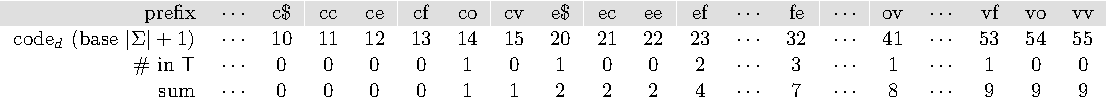
\includegraphics{kapitel/saca_algorithmen/bpr/algorithmus/phase1/bkt/image.pdf}
	}
	\caption[Tabelle \emph{bkt} zur Bestimmung der Bucket-Größen und -Positionen]{Tabelle \emph{bkt} zur Bestimmung der Bucket-Größen und -Positionen. Die Anzahl der Vorkommen eines Präfix im Text ist in Zeile 2 angegeben. Zeile 3 beinhaltet die kumulierte Anzahl und bestimmt damit die linke Grenze des nachfolgenden Buckets.}
	\label{fig:bkt}
\end{figure}
Der entsprechende Stand der Verarbeitung für den Text \(\inputtext = \covfefefe\) ist in Abbildung \ref{fig:bkt} zu sehen. Die kumulierte Größe aller Buckets bis einschließlich Bucket \(j\) legt gleichzeitig die linke Grenze des Buckets \(j+1\) fest. In einem weiteren Durchlauf können jetzt alle Suffixe \(\suffix{0}, \ldots, \suffix{n-1}\) im vorläufigen Suffixarray \sa einsortiert werden. Das Suffixarray beinhaltet dabei für ein Suffix \suffix{i} mit \(0 \leq i < n\) nicht das gesamte Suffix als String, sondern lediglich den Index \(i\) des Suffixes. Abbildung \ref{fig:buckets_initial} zeigt die initiale Einteilung der Buckets für \(d=2\). Zur besseren Visualisierung sind hier in dem Array die Suffixe anstatt der bloßen Indizes angegeben.\par\smallskip
\begin{figure}[ht]
	\resizebox{\textwidth}{!}{
		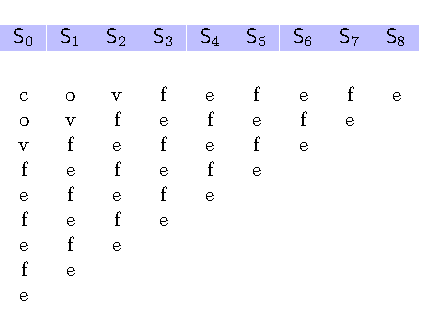
\includegraphics{kapitel/saca_algorithmen/bpr/algorithmus/phase1/sa_initial/image.pdf}
		\hspace{1em}
		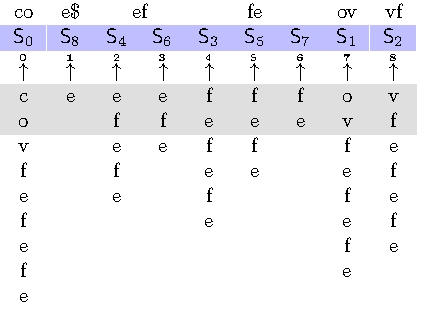
\includegraphics{kapitel/saca_algorithmen/bpr/algorithmus/phase1/buckets_initial/image.pdf}
	}
	\caption[Suffixe unsortiert und nach der ersten Phase des Algorithmus]{Suffixe unsortiert (links) und nach der ersten Phase des Algorithmus (rechts)}
	\label{fig:buckets_initial}
\end{figure}
Wie bereits zuvor erwähnt, wollen wir in der zweiten Phase des Algorithmus die Buckets verfeinern, indem eine weitere Gruppierung jedes bestehenden Buckets aufgebaut wird.\par
\begin{wrapfigure}[15]{r}{0.42\textwidth}
	\vspace{-1em}
	\resizebox{0.42\textwidth}{!}{
		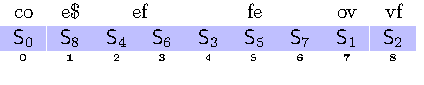
\includegraphics{kapitel/saca_algorithmen/bpr/algorithmus/phase1/buckets_initial_plain/image.pdf}
	}\\
	\resizebox{0.42\textwidth}{!}{
		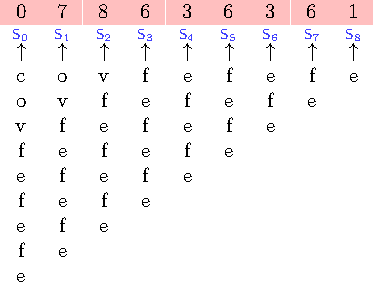
\includegraphics{kapitel/saca_algorithmen/bpr/algorithmus/phase1/bptr_initial/image.pdf}
	}
	\caption[Vorsortierte Suffixe und zugehörige Bucket-Pointer]{Vorsortierte Suffixe und zugehörige Bucket-Pointer}
	\label{fig:bucket_pointer_initial}
\end{wrapfigure}
Wir wollen dazu auf die bereits bekannte Einteilung der Suffixe in Level-\(d\)-Buckets zugreifen und anhand dessen eine weiterführende Sortierung vollziehen. Eine Anfrage, in welchem Bucket sich ein Suffix befindet, ist jedoch mit der bisher eingeführten Datenstruktur nicht effizient zu beantworten. \par
Es wird daher mit dem Bucket Pointer \bptr ein zweites Array eingeführt, welches sinngemäß ein Reverse Mapping des Suffixarrays \sa beinhaltet (s. Abbildung \ref{fig:bucket_pointer_initial}). In diesem Array symbolisiert jeder Index ein Suffix, wobei der Eintrag \(\bptr[i]\) den zugehörigen Bucket angibt, welcher jeweils über seine rechte Grenze identifiziert wird. Die Bestimmung der Grenzen erfolgt durch Ablesen der kumulierten Summe aus der Tabelle \bkt.
